\documentclass[final]{beamer}



% global default settings
%\usepackage[orientation=landscape, scale=0.6, size=custom, height=60.96, width=91.44, debug]{beamerposter}
\usepackage[orientation=landscape, scale=0.68, size=custom, height=50, width=70, debug]{beamerposter}
\usetheme{confposter}
	\setbeamercolor{block title}{fg=cardinalred, bg=white}
	\setbeamercolor{block body}{fg=black, bg=white}
	\setbeamercolor{block alerted title}{fg=white, bg=cardinalred}
	\setbeamercolor{block alerted body}{fg=Black, bg=cloud}
\usepackage[font=small,labelfont=bf]{caption}
\captionsetup[figure]{labelformat=simple}
\captionsetup[table]{labelformat=simple}

\usepackage{tabularx}
\newcolumntype{C}[1]{>{\centering\arraybackslash}p{#1}}
\usepackage{wrapfig}


% layout
% You can set your column widths, spacings, etc. here
% \setlength{\paperwidth}{36in}
% \setlength{\paperheight}{24in}
\newlength{\sepwid}
\setlength{\sepwid}{0.02\paperwidth}
\newlength{\firstcolwid}
\setlength{\firstcolwid}{0.20\paperwidth}
\newlength{\secondcolwid}
\setlength{\secondcolwid}{0.25\paperwidth}
\newlength{\thirdcolwid}
\setlength{\thirdcolwid}{0.25\paperwidth}
\newlength{\lastcolwid}
\setlength{\lastcolwid}{0.20\paperwidth}
\setlength{\topmargin}{-0.5in}

\addtobeamertemplate{block end}{}{\vspace*{1em}}
\addtobeamertemplate{block alerted end}{}{\vspace*{1em}}

% indentation needs to be set-up manually
% (beamer ignores indentations by default)
\makeatletter \addtobeamertemplate{block begin}{}{\setlength{\parindent}{1cm}\@afterindentfalse\@afterheading} \makeatletter

\usepackage[english]{babel}
\usepackage{blindtext}
\usepackage[utf8]{inputenc}
\usepackage{amsmath, amsthm, amssymb, latexsym}
% \usepackage[justification=centering,labelformat=empty]{caption}
% \captionsetup{font={rm}}
\usepackage{graphicx}
% \usepackage{moresize}
\usepackage{fix-cm}
\newcommand{\HUGE}{\fontsize{45}{54}\selectfont}
% \makeatletter
% \newcommand\HUGE{\@setfontsize\Huge{}{80}}
% \makeatother  
\usepackage{url}
\usepackage{tikz}
\usepackage{units}
\usepackage{changepage}
\usepackage{subcaption}
\usepackage{physics}
\usepackage{empheq}
\usepackage{tcolorbox}
\usepackage{natbib}

% make bibliography entries smaller
% \renewcommand\bibfont{\scriptsize}
% If you have more than one page of references, you want to tell beamer
% to put the continuation section label from the second slide onwards
\setbeamertemplate{frametitle continuation}[from second]
% Now get rid of all the colours
% (fancy colors in bibliography/reference is unnecessary...)
\setbeamercolor*{bibliography entry title}{fg=black}
\setbeamercolor*{bibliography entry author}{fg=black}
\setbeamercolor*{bibliography entry location}{fg=black}
\setbeamercolor*{bibliography entry note}{fg=black}
% and kill the abominable icon
\setbeamertemplate{bibliography item}{}

% Emphasize with Palo Alto Green
\newcommand{\emphg}[1]{{\color{paloalto}\textbf{#1}}}
% Emphasize with Cardinal Red
\newcommand{\emphr}[1]{{\color{cardinalred}\textbf{#1}}}




\title{
	\HUGE\color{cardinalred}
	A Machine Learning based Yelp Recommendation System
}
\author{
	\large{
	Pranav Bhardwaj\textsuperscript{1},
	Nicolas Bievre\textsuperscript{2},
	Frederik J. Mellbye\textsuperscript{3}\\
	\href{emailto:pranavb@stanford.edu}{\texttt{pranavb@stanford.edu}},
	\href{emailto:nbievre@stanford.edu}{\texttt{nbievre@stanford.edu}},
	\href{emailto:frederme@stanford.edu}{\texttt{frederme@stanford.edu}}
	}
}
\institute{
	\large{
	Department of Statistics, Stanford University\textsuperscript{1,2}	\\
	Institute for Computational and Mathematical Engineering, Stanford University\textsuperscript{3}
	}
}
\date{\today}


\begin{document}
\addtobeamertemplate{headline}{} 
{
	\begin{tikzpicture}[remember picture, overlay]
	% logo at top left corner
	\node [anchor=north west, inner sep=2cm]  at (current page.north west)
	{
\includegraphics[height=8cm]{./img/SU_Seal_Red.png}};
	\end{tikzpicture}
	\begin{tikzpicture}[remember picture, overlay]
	% logo at top right corner
     \node [anchor=north east, inner sep=2cm, yshift=-1.15cm]  at (current page.north east)
     {
\includegraphics[height=5cm]{./img/yelp.png}};
 \end{tikzpicture}
%  \begin{tikzpicture}[remember picture, overlay]
% 	% logo at top right corner
%      \node [anchor=north west, inner sep=2cm]  at (current page.north east)
%      {
\includegraphics[height=5.5cm]{./img/ICME.gif}};
%  \end{tikzpicture}
 }
\begin{frame}[t]



% Start your poster contents below the title

\begin{columns}[t]

\begin{column}{\sepwid}\end{column}

\begin{column}{\firstcolwid}

	\begin{alertblock}{\textbf{Abstract}}
		
% 		Briefly explain the motivation for your topic, what you built, and the results. It's easier to think of this as a quick summary of the inputs and outputs (5 sentences max)

    The Yelp Open Challenge data set contains user, business, and review data from 2004 to 2018. Binary classification is performed using user and business features to predict positive labels of 5 star ratings. High predicted probabilities correspond to recommendations. Linear and tree based models were used. Tree based models performed well due in part to their ability to represent nonlinear relationships. Models generalized well to the future. 
	\end{alertblock}
	
    \begin{block}{Data}
        % Exactly where did your data come from and what does your contain? (ie. what are in the rows and columns? Are examples labeled with ground truth? (2-3 sentences max)
         Each row corresponds to a review containing user and business information. The label $y$ is positive ($1$) if the user $u$ left the business $b$ as $5$ star review, and negative ($0$) otherwise.
        
        \begin{table}
        \centering
        \caption{Train-Validation-Test Split}
        \label{tab:split}
        \vspace{-1em}
        \begin{tabular}{lllll}
            \hline
                       & Reviews   & Users     & Businesses & 5 \bigstar \\ \hline
            Train      &4,903,362 & 1,259,558 & 125,159    & 43.1\%            \\
            Validation &527,276   & 262,764   & 75,605     & 51.5\%            \\
            Test       &527,276   & 274,722   & 75,254     & 51.8\%           
        \end{tabular}
        \end{table}
    \end{block}
    \vspace{-0.7em}
    \begin{block}{Features}
    
    % How many features do you have and which features are the raw input data (ex. color, weight, location, etc) vs. features you have derived (ex. ICA, Gaussian Kernel)? Why they are appropriate for this task? ​(3-4 sentences max)
    Input information to learning algorithms, $x$, is a concatenation of the user features, $x_u$, and the business features $x_b$. A single example $i$ is then:

\begin{align}
    \begin{bmatrix} x^{(i)}_u \\ x^{(i)}_b \end{bmatrix} = x^{(i)} \in \mathcal{R}^d,  y^{(i)} \in \{0, 1 \}
\end{align}

Where $d = 166$ is the number of predictors.
    \end{block}

\end{column}

\begin{column}{\sepwid}\end{column}

%\vspace{-1em}
\begin{column}[t]{\secondcolwid}
\begin{block}{Models}
    %   Exactly which model(s) are you using? Write out the basic math formulas and clearly note any modifications or
    %   additions. If you have more than one model, make subsections for each. (3-4 sentences max)
    {\color{cardinalred}\textbf{Logistic regression}:}\\ \noindent
    In logistic regression, the predicted probability of a $5$ star rating is of the form:
    \begin{align}
        h_\theta (x) = g(\theta^Tx) = \frac{1}{1 + e^{- \theta^T x}}
    \end{align}
    Models are trained using $L_1$ and $L_2$ regularization with unit regularization strength. \vspace{1em}
    \\ \noindent
    {\color{cardinalred}\textbf{Gaussian Discriminant Analysis (GDA)}:}\\ \noindent
    In GDA, it is assumed that $p(x \mid y)$ follows a multivariate normal distribution.
    Model parameters $\phi, \mu_0, \mu_1$ and $\Sigma$ are fit by maximizing the log-likelihood of the data given by:
    \begin{align}
        \ell(\phi, \mu_0, \mu_1, \Sigma) = \log \prod_{i=1}^n p(x^{(i)} \mid y^{(i)}; \mu_0, \mu_1, \Sigma) p(y^{(i)}; \phi)
    \end{align}
    A linear decision boundary at which $p(y = 1 \mid x) = 0.5$ is created. \\
    \vspace{1em}
    \noindent
    {\color{cardinalred}\textbf{Tree based methods} \cite{ESL}:} \\
    \noindent
    \noindent {\color{cardinalred}\textit{Decision Trees:}}
    In Decision Trees, the input space $\mathcal{X}$ is repeatedly split into two child regions by thresholding a single feature. The work presented uses cross-entropy loss, which is of the form:
    \begin{align}
        L_{cross}(R) = - \sum_c \hat{p}_c \log_2 \hat{p}_c
    \end{align}
    The predictor split corresponding to the maximum reduction in loss is made at each step.
    
    \noindent {\color{cardinalred} \textit{Random Forests:}}
    Random Forest Classifiers are constructed by bagging Decision Tree Classifiers which are trained using a random subset of features. To predict on a new example, the majority vote from the Decision Tree Classifiers is returned.\vspace{0.5em}
    \noindent {\color{cardinalred} \textit{Adaboost:}}
    AdaBoost classifiers sequentially apply base classifiers $G_{m}(x)$ (here decision trees) to modified versions of the data. The initial version of the data has uniform weighting. In each successive iteration $m$, observation weights are modified to place more weight on examples misclassified by the previous classifier $G_{m-1}(x)$.
    \end{block}
	 
\end{column}

\begin{column}{\sepwid}\end{column}

\begin{column}[t]{\thirdcolwid}
	
	\begin{block}{Results}
	
% 	Make a compact table of results. Each row should be a different model. The columns should be the training error and
%     the test error. List how many samples are in each of the training and testing data sets. Obviously, these sets should be
%     different. (1-2 sentences max + 1 table max)

    Model selection was based on validation set accuracy, reported in Table~\ref{tab:results}.
    
    \begin{table}[]
    \centering
    \caption{Train and validation accuracy, implemented in \textit{scikit-learn} \cite{sklearn}}
    \label{tab:results}
    \begin{tabular}{lll}
        \hline
                                                & Train    & Validation \\ \hline
        $L_{2}$-regularized Logistic Regression & 63.73 \% & 60.53 \%   \\
        $L_{1}$-regularized Logistic Regression & 74.15 \% & 74.84 \%   \\
        GDA                                     & 74.07 \% & 74.69 \%   \\
        Decision tree                           & 75.37 \% & 75.97 \%   \\
        Random Forest                           & 71.58 \% & 71.56 \%   \\
        AdaBoost                                & 75.33 \% & 76.13 \%   \\ \hline
    \end{tabular}
    \end{table}
    \vspace{1.2em}
    The final model selected was an AdaBoost classifier with $40$ base estimators. Each base estimator was a decision tree classifiers of maximum depth $4$. Test set performance is summarized in Figure~\ref{fig:roc} and Table~\ref{tab:adaboost}.
    \vspace{1.2em}
    \begin{figure}
        \hbox{\hspace{-1em}
        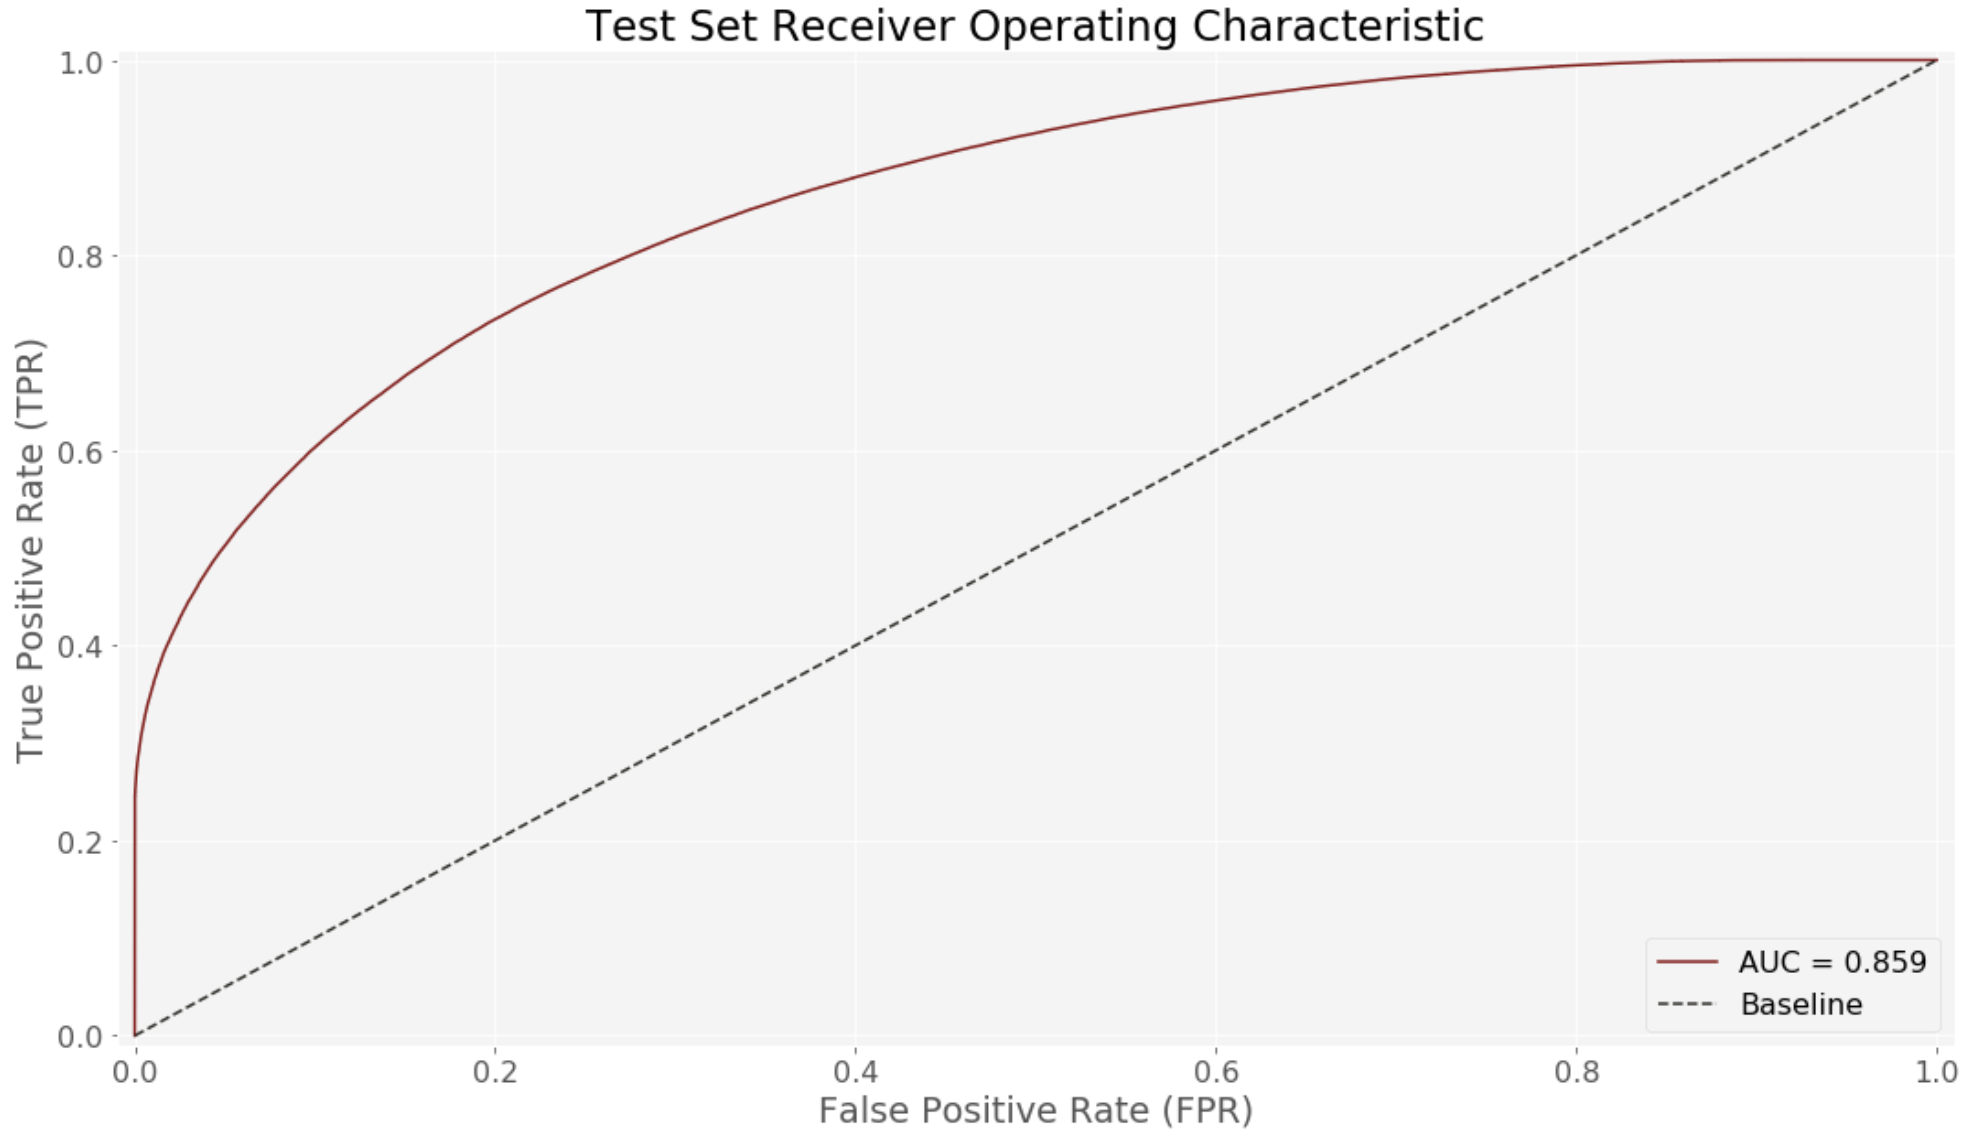
\includegraphics[width=1.05\thirdcolwid]{./img/roc.png}}
        \caption{Test set AUC-ROC curve for the AdaBoost classifier}
        \label{fig:roc}
    \end{figure}
    
    \begin{table}[]
    \centering
    \caption{AdaBoost classifier test set performance}
    \label{tab:adaboost}
    \begin{tabular}{lllll}
        \hline
        & Accuracy & Precision & Recall & F1 \\ \hline
        AdaBoost & 76.63 \%   & 79.18 \% & 74.53 \% & 76.78 \% \\ 
    \end{tabular}
    \end{table}

	\end{block}
	
\end{column}

\begin{column}{\sepwid}\end{column}

\begin{column}[t]{\lastcolwid}
	
	\begin{block}{Discussion}
		% This is where you share your thoughts about your project. (Hopefully you have a few interesting interpretations!) Briefly summarized what just happened. Briefly explain whether or not you expected your results. If your results were good, explain why. If they were not good, explain why. (6 sentences max)
		
		Logistic regression with $L_1$ regularization as well as tree based methods performed and generalized to future data well. We believe this is because these models effectively use a subset of predictors, and many predictors are not adding useful signal. This would also explain the poor performance of logistic regression with $L_2$ regularization. After cross-validation for model selection, an AdaBoost classifier with 40 base estimators, each a decision tree classifier with maximum depth 4, was deployed on the most recent data available. This model performed even better on test data than validation data. 
	\end{block}
	
	\begin{block}{Future Directions}
% 		If you had another 6 months to work on this, what would you do first? (2-3 sentences max)
\begin{itemize}
    \item Perform more extensive feature engineering
    \item Leverage more of the available Yelp data (tips, review text, photos)
    \item Leverage the community structure in Yelp with collaborative filtering and graph based models
    \item Provide recommendations to businesses on improvements they can make
\end{itemize}
	\end{block}
    
    \begin{block}{References}
		{\small
			\bibliographystyle{abbrv}
            %\bibliographystyle{acm}
		\bibliography{./bibliography}
		}
	\end{block}
\end{column}

\begin{column}{\sepwid}\end{column}

\end{columns}
\end{frame}
\end{document}